\subsection{Class Diagram}
This section will explain the most notable classes illustrated in \cref{fig:class} and its relations.

The \emph{Coordinate} trait models a geographic location on the earth. Because many functions are dealing with objects that can have coordinates, we can let these objects implement the \emph{Coordinate} trait, and thereby write these functions in a polymorphic way. One such object is the \emph{Position} class, which is essentially a coordinate for a person at a given time. \emph{ConfidencePosition} is designed to have the same structure as positions received from the aSTEP server, so when hopMap request position data a list of \emph{ConfidencePosition} will be returned. A \emph{ConfidencePosition} therefor also includes information about the certainty of a position, called Confidence as shown on \cref{fig:class}. This confidence is a distance which the position at most is offset from. \emph{ConfidencePosition} also has a \emph{lastLocatedTime} which is a time stamp for when the position was recorded by the aSTEP server.


The \emph{Person} class is a abstract class, defining methods which should be implemented in specialisations of this class, in order to enforce code reuse and consistency. The class contains the person's history of positions as an iterateable collection of the generic type \emph{T}. The generic type parameter \emph{T} is bounded to be a class implementing \emph{Coordinate}, denoted by \emph{T < Coordinate}. This prevents any specialisation of \emph{Person} from having a history of positions that is not a collection of \emph{Coordinate}s. \emph{T} is in a contravariant position, denoted by \emph{-T}, permitting specialisations of the \emph{Person} class to use a specialisation of \emph{T}. Contravariance allows the \emph{Person} class to have methods that takes an input of type \emph{T}, but excludes the class from defining methods which returns a \emph{T}. The most important method in the \emph{Person} class is \emph{movePerson}, which takes a \emph{T} and a \emph{DateTime} as parameters. Here the parameter of type \emph{T} is the location the person should be moved to, and the DateTime parameter is the time where the person arrived at the location. This method updates a person's history of positions to include the new position. Upon updating a person's history of positions, positions older than \emph{x} is removed from the person, where \emph{x} is a constant defined for all persons. To calculate a person's velocity and heading direction this history of positions is essential. 

\emph{Area} is the class representing a geographical area on a map. The most important method such a class should implement is the function \emph{isWithinArea} which taskes an input of type p:Coordinate):Bool

\begin{sidewaysfigure}[htbp]
\centering
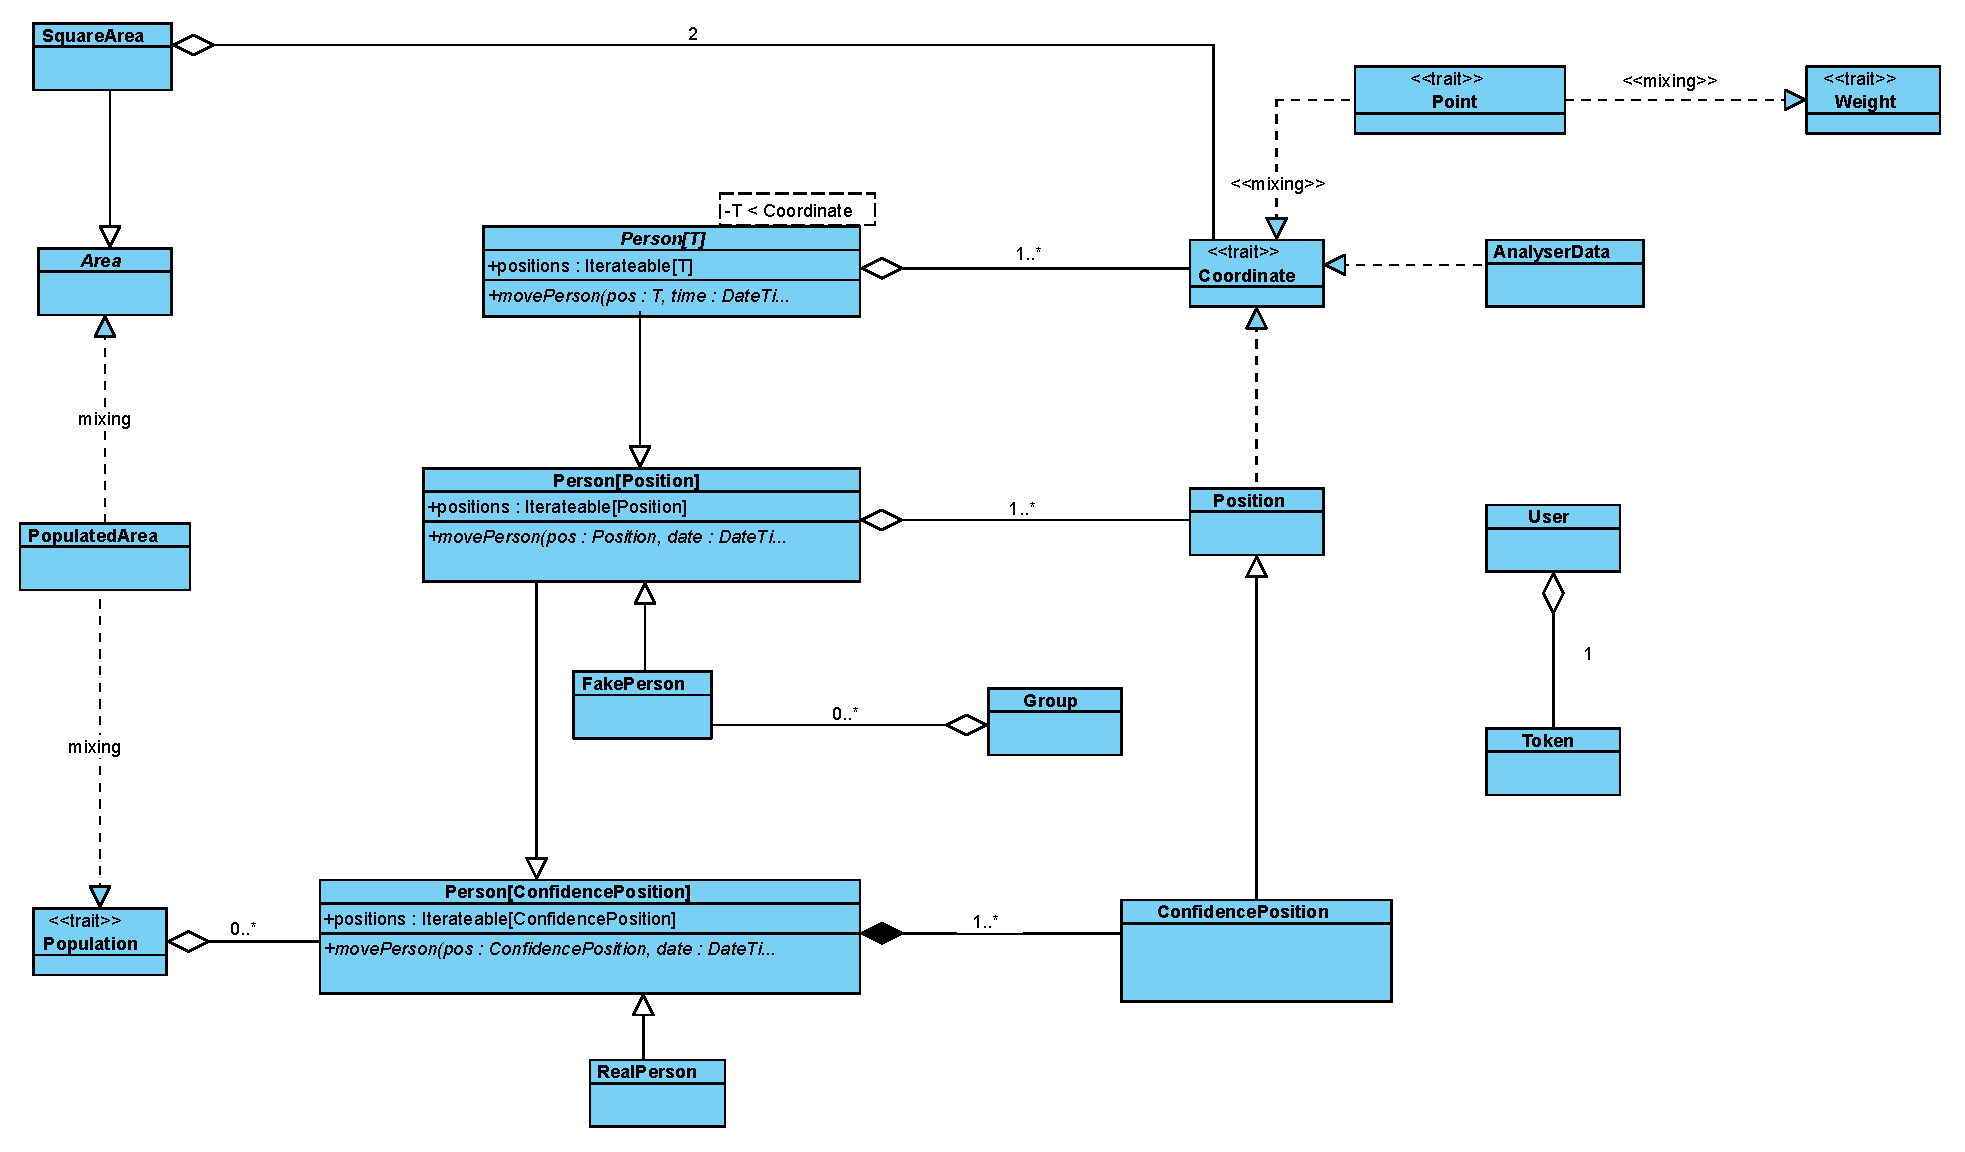
\includegraphics[width=\linewidth]{figures/class.eps}
\caption{Class diagram.}
\label{fig:class}
\end{sidewaysfigure}
